\documentclass[1p]{elsarticle_modified}
%\bibliographystyle{elsarticle-num}

%\usepackage[colorlinks]{hyperref}
%\usepackage{abbrmath_seonhwa} %\Abb, \Ascr, \Acal ,\Abf, \Afrak
\usepackage{amsfonts}
\usepackage{amssymb}
\usepackage{amsmath}
\usepackage{amsthm}
\usepackage{scalefnt}
\usepackage{amsbsy}
\usepackage{kotex}
\usepackage{caption}
\usepackage{subfig}
\usepackage{color}
\usepackage{graphicx}
\usepackage{xcolor} %% white, black, red, green, blue, cyan, magenta, yellow
\usepackage{float}
\usepackage{setspace}
\usepackage{hyperref}

\usepackage{tikz}
\usetikzlibrary{arrows}

\usepackage{multirow}
\usepackage{array} % fixed length table
\usepackage{hhline}

%%%%%%%%%%%%%%%%%%%%%
\makeatletter
\renewcommand*\env@matrix[1][\arraystretch]{%
	\edef\arraystretch{#1}%
	\hskip -\arraycolsep
	\let\@ifnextchar\new@ifnextchar
	\array{*\c@MaxMatrixCols c}}
\makeatother %https://tex.stackexchange.com/questions/14071/how-can-i-increase-the-line-spacing-in-a-matrix
%%%%%%%%%%%%%%%

\usepackage[normalem]{ulem}

\newcommand{\msout}[1]{\ifmmode\text{\sout{\ensuremath{#1}}}\else\sout{#1}\fi}
%SOURCE: \msout is \stkout macro in https://tex.stackexchange.com/questions/20609/strikeout-in-math-mode

\newcommand{\cancel}[1]{
	\ifmmode
	{\color{red}\msout{#1}}
	\else
	{\color{red}\sout{#1}}
	\fi
}

\newcommand{\add}[1]{
	{\color{blue}\uwave{#1}}
}

\newcommand{\replace}[2]{
	\ifmmode
	{\color{red}\msout{#1}}{\color{blue}\uwave{#2}}
	\else
	{\color{red}\sout{#1}}{\color{blue}\uwave{#2}}
	\fi
}

\newcommand{\Sol}{\mathcal{S}} %segment
\newcommand{\D}{D} %diagram
\newcommand{\A}{\mathcal{A}} %arc


%%%%%%%%%%%%%%%%%%%%%%%%%%%%%5 test

\def\sl{\operatorname{\textup{SL}}(2,\Cbb)}
\def\psl{\operatorname{\textup{PSL}}(2,\Cbb)}
\def\quan{\mkern 1mu \triangleright \mkern 1mu}

\theoremstyle{definition}
\newtheorem{thm}{Theorem}[section]
\newtheorem{prop}[thm]{Proposition}
\newtheorem{lem}[thm]{Lemma}
\newtheorem{ques}[thm]{Question}
\newtheorem{cor}[thm]{Corollary}
\newtheorem{defn}[thm]{Definition}
\newtheorem{exam}[thm]{Example}
\newtheorem{rmk}[thm]{Remark}
\newtheorem{alg}[thm]{Algorithm}

\newcommand{\I}{\sqrt{-1}}
\begin{document}

%\begin{frontmatter}
%
%\title{Boundary parabolic representations of knots up to 8 crossings}
%
%%% Group authors per affiliation:
%\author{Yunhi Cho} 
%\address{Department of Mathematics, University of Seoul, Seoul, Korea}
%\ead{yhcho@uos.ac.kr}
%
%
%\author{Seonhwa Kim} %\fnref{s_kim}}
%\address{Center for Geometry and Physics, Institute for Basic Science, Pohang, 37673, Korea}
%\ead{ryeona17@ibs.re.kr}
%
%\author{Hyuk Kim}
%\address{Department of Mathematical Sciences, Seoul National University, Seoul 08826, Korea}
%\ead{hyukkim@snu.ac.kr}
%
%\author{Seokbeom Yoon}
%\address{Department of Mathematical Sciences, Seoul National University, Seoul, 08826,  Korea}
%\ead{sbyoon15@snu.ac.kr}
%
%\begin{abstract}
%We find all boundary parabolic representation of knots up to 8 crossings.
%
%\end{abstract}
%\begin{keyword}
%    \MSC[2010] 57M25 
%\end{keyword}
%
%\end{frontmatter}

%\linenumbers
%\tableofcontents
%
\newcommand\colored[1]{\textcolor{white}{\rule[-0.35ex]{0.8em}{1.4ex}}\kern-0.8em\color{red} #1}%
%\newcommand\colored[1]{\textcolor{white}{ #1}\kern-2.17ex	\textcolor{white}{ #1}\kern-1.81ex	\textcolor{white}{ #1}\kern-2.15ex\color{red}#1	}

{\Large $\underline{12n_{0777}~(K12n_{0777})}$}

\setlength{\tabcolsep}{10pt}
\renewcommand{\arraystretch}{1.6}
\vspace{1cm}\begin{tabular}{m{100pt}>{\centering\arraybackslash}m{274pt}}
\multirow{5}{120pt}{
	\centering
	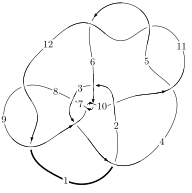
\includegraphics[width=112pt]{../../../GIT/diagram.site/Diagrams/png/2866_12n_0777.png}\\
\ \ \ A knot diagram\footnotemark}&
\allowdisplaybreaks
\textbf{Linearized knot diagam} \\
\cline{2-2}
 &
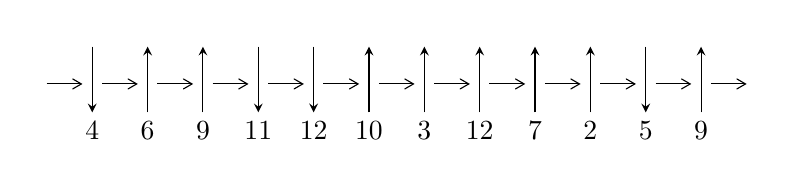
\begin{tikzpicture}[x=20pt, y=17pt]
	% nodes
	\node (C0) at (0, 0) {};
	\node (C1) at (1, 0) {};
	\node (C1U) at (1, +1) {};
	\node (C1D) at (1, -1) {4};

	\node (C2) at (2, 0) {};
	\node (C2U) at (2, +1) {};
	\node (C2D) at (2, -1) {6};

	\node (C3) at (3, 0) {};
	\node (C3U) at (3, +1) {};
	\node (C3D) at (3, -1) {9};

	\node (C4) at (4, 0) {};
	\node (C4U) at (4, +1) {};
	\node (C4D) at (4, -1) {11};

	\node (C5) at (5, 0) {};
	\node (C5U) at (5, +1) {};
	\node (C5D) at (5, -1) {12};

	\node (C6) at (6, 0) {};
	\node (C6U) at (6, +1) {};
	\node (C6D) at (6, -1) {10};

	\node (C7) at (7, 0) {};
	\node (C7U) at (7, +1) {};
	\node (C7D) at (7, -1) {3};

	\node (C8) at (8, 0) {};
	\node (C8U) at (8, +1) {};
	\node (C8D) at (8, -1) {12};

	\node (C9) at (9, 0) {};
	\node (C9U) at (9, +1) {};
	\node (C9D) at (9, -1) {7};

	\node (C10) at (10, 0) {};
	\node (C10U) at (10, +1) {};
	\node (C10D) at (10, -1) {2};

	\node (C11) at (11, 0) {};
	\node (C11U) at (11, +1) {};
	\node (C11D) at (11, -1) {5};

	\node (C12) at (12, 0) {};
	\node (C12U) at (12, +1) {};
	\node (C12D) at (12, -1) {9};
	\node (C13) at (13, 0) {};

	% arrows
	\draw[->,>={angle 60}]
	(C0) edge (C1) (C1) edge (C2) (C2) edge (C3) (C3) edge (C4) (C4) edge (C5) (C5) edge (C6) (C6) edge (C7) (C7) edge (C8) (C8) edge (C9) (C9) edge (C10) (C10) edge (C11) (C11) edge (C12) (C12) edge (C13) ;	\draw[->,>=stealth]
	(C1U) edge (C1D) (C2D) edge (C2U) (C3D) edge (C3U) (C4U) edge (C4D) (C5U) edge (C5D) (C6D) edge (C6U) (C7D) edge (C7U) (C8D) edge (C8U) (C9D) edge (C9U) (C10D) edge (C10U) (C11U) edge (C11D) (C12D) edge (C12U) ;
	\end{tikzpicture} \\
\hhline{~~} \\& 
\textbf{Solving Sequence} \\ \cline{2-2} 
 &
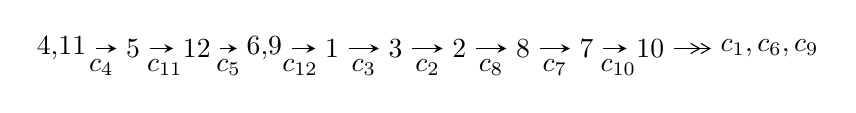
\begin{tikzpicture}[x=23pt, y=7pt]
	% node
	\node (A0) at (-1/8, 0) {4,11};
	\node (A1) at (1, 0) {5};
	\node (A2) at (2, 0) {12};
	\node (A3) at (49/16, 0) {6,9};
	\node (A4) at (33/8, 0) {1};
	\node (A5) at (41/8, 0) {3};
	\node (A6) at (49/8, 0) {2};
	\node (A7) at (57/8, 0) {8};
	\node (A8) at (65/8, 0) {7};
	\node (A9) at (73/8, 0) {10};
	\node (C1) at (1/2, -1) {$c_{4}$};
	\node (C2) at (3/2, -1) {$c_{11}$};
	\node (C3) at (5/2, -1) {$c_{5}$};
	\node (C4) at (29/8, -1) {$c_{12}$};
	\node (C5) at (37/8, -1) {$c_{3}$};
	\node (C6) at (45/8, -1) {$c_{2}$};
	\node (C7) at (53/8, -1) {$c_{8}$};
	\node (C8) at (61/8, -1) {$c_{7}$};
	\node (C9) at (69/8, -1) {$c_{10}$};
	\node (A10) at (11, 0) {$c_{1},c_{6},c_{9}$};

	% edge
	\draw[->,>=stealth]	
	(A0) edge (A1) (A1) edge (A2) (A2) edge (A3) (A3) edge (A4) (A4) edge (A5) (A5) edge (A6) (A6) edge (A7) (A7) edge (A8) (A8) edge (A9) ;
	\draw[->>,>={angle 60}]	
	(A9) edge (A10);
\end{tikzpicture} \\ 

\end{tabular} \\

\footnotetext{
The image of knot diagram is generated by the software ``\textbf{Draw programme}" developed by Andrew Bartholomew(\url{http://www.layer8.co.uk/maths/draw/index.htm\#Running-draw}), where we modified some parts for our purpose(\url{https://github.com/CATsTAILs/LinksPainter}).
}\phantom \\ \newline 
\centering \textbf{Ideals for irreducible components\footnotemark of $X_{\text{par}}$} 
 
\begin{align*}
I^u_{1}&=\langle 
4585 u^{29}-53373 u^{28}+\cdots+32 b-211552,\;13955 u^{29}-160849 u^{28}+\cdots+64 a-593856,\\
\phantom{I^u_{1}}&\phantom{= \langle  }u^{30}-13 u^{29}+\cdots-96 u+64\rangle \\
I^u_{2}&=\langle 
3 u^{21}-2 u^{20}+\cdots+b+1,\;5 u^{21}-6 u^{20}+\cdots+a+4,\;u^{22}-12 u^{20}+\cdots+2 u+1\rangle \\
I^u_{3}&=\langle 
-8.71806\times10^{22} a^{11} u+1.90564\times10^{22} a^{10} u+\cdots+4.42015\times10^{24} a+2.07365\times10^{24},\\
\phantom{I^u_{3}}&\phantom{= \langle  }- a^{11} u-8 a^{10} u+\cdots-155 a+597,\;u^2+u-1\rangle \\
\\
\end{align*}
\raggedright * 3 irreducible components of $\dim_{\mathbb{C}}=0$, with total 76 representations.\\
\footnotetext{All coefficients of polynomials are rational numbers. But the coefficients are sometimes approximated in decimal forms when there is not enough margin.}
\newpage
\renewcommand{\arraystretch}{1}
\centering \section*{I. $I^u_{1}= \langle 4585 u^{29}-53373 u^{28}+\cdots+32 b-211552,\;13955 u^{29}-160849 u^{28}+\cdots+64 a-593856,\;u^{30}-13 u^{29}+\cdots-96 u+64 \rangle$}
\flushleft \textbf{(i) Arc colorings}\\
\begin{tabular}{m{7pt} m{180pt} m{7pt} m{180pt} }
\flushright $a_{4}=$&$\begin{pmatrix}1\\0\end{pmatrix}$ \\
\flushright $a_{11}=$&$\begin{pmatrix}0\\u\end{pmatrix}$ \\
\flushright $a_{5}=$&$\begin{pmatrix}1\\u^2\end{pmatrix}$ \\
\flushright $a_{12}=$&$\begin{pmatrix}- u\\- u^3+u\end{pmatrix}$ \\
\flushright $a_{6}=$&$\begin{pmatrix}- u^2+1\\- u^4+2 u^2\end{pmatrix}$ \\
\flushright $a_{9}=$&$\begin{pmatrix}-218.047 u^{29}+2513.27 u^{28}+\cdots-7883.75 u+9279\\-143.281 u^{29}+1667.91 u^{28}+\cdots-5240.50 u+6611\end{pmatrix}$ \\
\flushright $a_{1}=$&$\begin{pmatrix}-12 u^{29}+\frac{583}{4} u^{28}+\cdots-\frac{961}{2} u+\frac{1409}{2}\\\frac{31}{4} u^{29}-\frac{325}{4} u^{28}+\cdots+\frac{465}{2} u-112\end{pmatrix}$ \\
\flushright $a_{3}=$&$\begin{pmatrix}12 u^{29}-\frac{583}{4} u^{28}+\cdots+\frac{959}{2} u-\frac{1407}{2}\\-\frac{31}{4} u^{29}+\frac{325}{4} u^{28}+\cdots-\frac{463}{2} u+112\end{pmatrix}$ \\
\flushright $a_{2}=$&$\begin{pmatrix}-\frac{79}{4} u^{29}+227 u^{28}+\cdots-713 u+\frac{1633}{2}\\\frac{31}{4} u^{29}-\frac{325}{4} u^{28}+\cdots+\frac{465}{2} u-112\end{pmatrix}$ \\
\flushright $a_{8}=$&$\begin{pmatrix}-412.797 u^{29}+4786.39 u^{28}+\cdots-15027.8 u+18449\\-282.531 u^{29}+3320.78 u^{28}+\cdots-10460.5 u+13993\end{pmatrix}$ \\
\flushright $a_{7}=$&$\begin{pmatrix}-\frac{1425}{8} u^{29}+\frac{32277}{16} u^{28}+\cdots-6300 u+6463\\-\frac{3901}{16} u^{29}+\frac{5761}{2} u^{28}+\cdots-9090 u+12556\end{pmatrix}$ \\
\flushright $a_{10}=$&$\begin{pmatrix}-\frac{77}{4} u^{29}+\frac{825}{4} u^{28}+\cdots-\frac{2465}{4} u+368\\-90 u^{29}+\frac{4209}{4} u^{28}+\cdots-3335 u+4240\end{pmatrix}$\\&\end{tabular}
\flushleft \textbf{(ii) Obstruction class $= -1$}\\~\\
\flushleft \textbf{(iii) Cusp Shapes $= -\frac{3861}{4} u^{29}+\frac{22479}{2} u^{28}+\cdots-35492 u+44366$}\\~\\
\newpage\renewcommand{\arraystretch}{1}
\flushleft \textbf{(iv) u-Polynomials at the component}\newline \\
\begin{tabular}{m{50pt}|m{274pt}}
Crossings & \hspace{64pt}u-Polynomials at each crossing \\
\hline $$\begin{aligned}c_{1}\end{aligned}$$&$\begin{aligned}
&u^{30}-14 u^{29}+\cdots-1674 u+180
\end{aligned}$\\
\hline $$\begin{aligned}c_{2},c_{10}\end{aligned}$$&$\begin{aligned}
&u^{30}- u^{29}+\cdots-4 u+1
\end{aligned}$\\
\hline $$\begin{aligned}c_{3},c_{8},c_{12}\end{aligned}$$&$\begin{aligned}
&u^{30}+25 u^{28}+\cdots+14 u^2+1
\end{aligned}$\\
\hline $$\begin{aligned}c_{4},c_{5},c_{11}\end{aligned}$$&$\begin{aligned}
&u^{30}-13 u^{29}+\cdots-96 u+64
\end{aligned}$\\
\hline $$\begin{aligned}c_{6},c_{9}\end{aligned}$$&$\begin{aligned}
&u^{30}+9 u^{29}+\cdots+58 u+4
\end{aligned}$\\
\hline $$\begin{aligned}c_{7}\end{aligned}$$&$\begin{aligned}
&u^{30}+u^{29}+\cdots+134 u+43
\end{aligned}$\\
\hline
\end{tabular}\\~\\
\newpage\renewcommand{\arraystretch}{1}
\flushleft \textbf{(v) Riley Polynomials at the component}\newline \\
\begin{tabular}{m{50pt}|m{274pt}}
Crossings & \hspace{64pt}Riley Polynomials at each crossing \\
\hline $$\begin{aligned}c_{1}\end{aligned}$$&$\begin{aligned}
&y^{30}-42 y^{29}+\cdots-660636 y+32400
\end{aligned}$\\
\hline $$\begin{aligned}c_{2},c_{10}\end{aligned}$$&$\begin{aligned}
&y^{30}+27 y^{29}+\cdots+10 y+1
\end{aligned}$\\
\hline $$\begin{aligned}c_{3},c_{8},c_{12}\end{aligned}$$&$\begin{aligned}
&y^{30}+50 y^{29}+\cdots+28 y+1
\end{aligned}$\\
\hline $$\begin{aligned}c_{4},c_{5},c_{11}\end{aligned}$$&$\begin{aligned}
&y^{30}-27 y^{29}+\cdots+7168 y+4096
\end{aligned}$\\
\hline $$\begin{aligned}c_{6},c_{9}\end{aligned}$$&$\begin{aligned}
&y^{30}+21 y^{29}+\cdots-204 y+16
\end{aligned}$\\
\hline $$\begin{aligned}c_{7}\end{aligned}$$&$\begin{aligned}
&y^{30}+37 y^{29}+\cdots-12796 y+1849
\end{aligned}$\\
\hline
\end{tabular}\\~\\
\newpage\flushleft \textbf{(vi) Complex Volumes and Cusp Shapes}
$$\begin{array}{c|c|c}  
\text{Solutions to }I^u_{1}& \I (\text{vol} + \sqrt{-1}CS) & \text{Cusp shape}\\
 \hline 
\begin{aligned}
u &= -0.712100 + 0.956564 I \\
a &= \phantom{-}0.866632 - 0.189288 I \\
b &= -0.17533 - 2.06721 I\end{aligned}
 & -12.2909 + 9.4994 I & \phantom{-0.000000 } 0. - 5.67165 I \\ \hline\begin{aligned}
u &= -0.712100 - 0.956564 I \\
a &= \phantom{-}0.866632 + 0.189288 I \\
b &= -0.17533 + 2.06721 I\end{aligned}
 & -12.2909 - 9.4994 I & \phantom{-0.000000 -}0. + 5.67165 I \\ \hline\begin{aligned}
u &= \phantom{-}1.076880 + 0.516113 I \\
a &= \phantom{-}1.16983 + 0.89905 I \\
b &= -0.750113 + 0.531557 I\end{aligned}
 & -0.60829 - 5.16519 I & \phantom{-}7.68800 - 3.17301 I \\ \hline\begin{aligned}
u &= \phantom{-}1.076880 - 0.516113 I \\
a &= \phantom{-}1.16983 - 0.89905 I \\
b &= -0.750113 - 0.531557 I\end{aligned}
 & -0.60829 + 5.16519 I & \phantom{-}7.68800 + 3.17301 I \\ \hline\begin{aligned}
u &= -1.179430 + 0.197792 I \\
a &= -0.198189 + 0.197833 I \\
b &= -0.370253 + 0.632453 I\end{aligned}
 & -2.67535 + 1.28324 I & \phantom{-0.000000 } 0 \\ \hline\begin{aligned}
u &= -1.179430 - 0.197792 I \\
a &= -0.198189 - 0.197833 I \\
b &= -0.370253 - 0.632453 I\end{aligned}
 & -2.67535 - 1.28324 I & \phantom{-0.000000 } 0 \\ \hline\begin{aligned}
u &= -0.576495 + 1.064220 I \\
a &= \phantom{-}0.893792 - 0.009633 I \\
b &= -0.22203 - 2.04575 I\end{aligned}
 & -11.81400 - 2.89439 I & \phantom{-0.000000 } 0 \\ \hline\begin{aligned}
u &= -0.576495 - 1.064220 I \\
a &= \phantom{-}0.893792 + 0.009633 I \\
b &= -0.22203 + 2.04575 I\end{aligned}
 & -11.81400 + 2.89439 I & \phantom{-0.000000 } 0 \\ \hline\begin{aligned}
u &= -0.695385 + 1.054340 I \\
a &= -0.834599 + 0.093305 I \\
b &= \phantom{-}0.17902 + 2.11004 I\end{aligned}
 & -7.50297 + 3.48252 I & \phantom{-0.000000 } 0 \\ \hline\begin{aligned}
u &= -0.695385 - 1.054340 I \\
a &= -0.834599 - 0.093305 I \\
b &= \phantom{-}0.17902 - 2.11004 I\end{aligned}
 & -7.50297 - 3.48252 I & \phantom{-0.000000 } 0\\
 \hline 
 \end{array}$$\newpage$$\begin{array}{c|c|c}  
\text{Solutions to }I^u_{1}& \I (\text{vol} + \sqrt{-1}CS) & \text{Cusp shape}\\
 \hline 
\begin{aligned}
u &= \phantom{-}0.405900 + 0.604201 I \\
a &= -1.206390 - 0.215475 I \\
b &= \phantom{-}0.706818 + 0.267801 I\end{aligned}
 & \phantom{-}1.34273 + 0.69486 I & \phantom{-}10.73680 - 5.94826 I \\ \hline\begin{aligned}
u &= \phantom{-}0.405900 - 0.604201 I \\
a &= -1.206390 + 0.215475 I \\
b &= \phantom{-}0.706818 - 0.267801 I\end{aligned}
 & \phantom{-}1.34273 - 0.69486 I & \phantom{-}10.73680 + 5.94826 I \\ \hline\begin{aligned}
u &= -0.349023 + 0.634623 I \\
a &= \phantom{-}0.391030 + 0.430038 I \\
b &= \phantom{-}0.490044 - 0.392098 I\end{aligned}
 & -2.73365 + 3.23503 I & \phantom{-}0.14526 - 3.30647 I \\ \hline\begin{aligned}
u &= -0.349023 - 0.634623 I \\
a &= \phantom{-}0.391030 - 0.430038 I \\
b &= \phantom{-}0.490044 + 0.392098 I\end{aligned}
 & -2.73365 - 3.23503 I & \phantom{-}0.14526 + 3.30647 I \\ \hline\begin{aligned}
u &= -0.473468 + 0.455765 I \\
a &= \phantom{-}0.178820 - 0.624865 I \\
b &= -0.466864 - 0.464807 I\end{aligned}
 & -3.35774 + 0.41602 I & -0.28518 - 3.29821 I \\ \hline\begin{aligned}
u &= -0.473468 - 0.455765 I \\
a &= \phantom{-}0.178820 + 0.624865 I \\
b &= -0.466864 + 0.464807 I\end{aligned}
 & -3.35774 - 0.41602 I & -0.28518 + 3.29821 I \\ \hline\begin{aligned}
u &= -0.241152 + 0.560887 I \\
a &= -0.450417 + 0.043597 I \\
b &= \phantom{-}0.043133 + 0.373812 I\end{aligned}
 & \phantom{-}0.155530 + 1.274890 I & \phantom{-}2.11047 - 6.19395 I \\ \hline\begin{aligned}
u &= -0.241152 - 0.560887 I \\
a &= -0.450417 - 0.043597 I \\
b &= \phantom{-}0.043133 - 0.373812 I\end{aligned}
 & \phantom{-}0.155530 - 1.274890 I & \phantom{-}2.11047 + 6.19395 I \\ \hline\begin{aligned}
u &= \phantom{-}1.40597 + 0.22506 I \\
a &= \phantom{-}0.363023 + 0.409362 I \\
b &= \phantom{-}0.021884 + 0.360955 I\end{aligned}
 & -5.15833 - 4.20213 I & \phantom{-0.000000 } 0 \\ \hline\begin{aligned}
u &= \phantom{-}1.40597 - 0.22506 I \\
a &= \phantom{-}0.363023 - 0.409362 I \\
b &= \phantom{-}0.021884 - 0.360955 I\end{aligned}
 & -5.15833 + 4.20213 I & \phantom{-0.000000 } 0\\
 \hline 
 \end{array}$$\newpage$$\begin{array}{c|c|c}  
\text{Solutions to }I^u_{1}& \I (\text{vol} + \sqrt{-1}CS) & \text{Cusp shape}\\
 \hline 
\begin{aligned}
u &= \phantom{-}1.42237 + 0.17547 I \\
a &= \phantom{-}0.152611 - 0.928981 I \\
b &= \phantom{-}0.387688 - 0.480108 I\end{aligned}
 & -9.29324 - 2.70234 I & \phantom{-0.000000 } 0 \\ \hline\begin{aligned}
u &= \phantom{-}1.42237 - 0.17547 I \\
a &= \phantom{-}0.152611 + 0.928981 I \\
b &= \phantom{-}0.387688 + 0.480108 I\end{aligned}
 & -9.29324 + 2.70234 I & \phantom{-0.000000 } 0 \\ \hline\begin{aligned}
u &= \phantom{-}1.43366 + 0.23827 I \\
a &= -0.798085 + 0.019961 I \\
b &= -0.459766 - 0.343812 I\end{aligned}
 & -8.45070 - 6.42278 I & \phantom{-0.000000 } 0 \\ \hline\begin{aligned}
u &= \phantom{-}1.43366 - 0.23827 I \\
a &= -0.798085 - 0.019961 I \\
b &= -0.459766 + 0.343812 I\end{aligned}
 & -8.45070 + 6.42278 I & \phantom{-0.000000 } 0 \\ \hline\begin{aligned}
u &= \phantom{-}1.64901 + 0.32277 I \\
a &= -0.70265 - 1.71037 I \\
b &= \phantom{-}0.58983 - 2.17349 I\end{aligned}
 & \phantom{-}19.4368 - 14.3151 I & \phantom{-0.000000 } 0 \\ \hline\begin{aligned}
u &= \phantom{-}1.64901 - 0.32277 I \\
a &= -0.70265 + 1.71037 I \\
b &= \phantom{-}0.58983 + 2.17349 I\end{aligned}
 & \phantom{-}19.4368 + 14.3151 I & \phantom{-0.000000 } 0 \\ \hline\begin{aligned}
u &= \phantom{-}1.67171 + 0.34503 I \\
a &= \phantom{-}0.67299 + 1.59613 I \\
b &= -0.61499 + 2.14641 I\end{aligned}
 & -15.2886 - 8.7374 I & \phantom{-0.000000 } 0 \\ \hline\begin{aligned}
u &= \phantom{-}1.67171 - 0.34503 I \\
a &= \phantom{-}0.67299 - 1.59613 I \\
b &= -0.61499 - 2.14641 I\end{aligned}
 & -15.2886 + 8.7374 I & \phantom{-0.000000 } 0 \\ \hline\begin{aligned}
u &= \phantom{-}1.66154 + 0.39521 I \\
a &= -0.74838 - 1.46675 I \\
b &= \phantom{-}0.64093 - 2.07022 I\end{aligned}
 & -19.0732 - 2.6309 I & \phantom{-0.000000 } 0 \\ \hline\begin{aligned}
u &= \phantom{-}1.66154 - 0.39521 I \\
a &= -0.74838 + 1.46675 I \\
b &= \phantom{-}0.64093 + 2.07022 I\end{aligned}
 & -19.0732 + 2.6309 I & \phantom{-0.000000 } 0\\
 \hline 
 \end{array}$$\newpage\newpage\renewcommand{\arraystretch}{1}
\centering \section*{II. $I^u_{2}= \langle 3 u^{21}-2 u^{20}+\cdots+b+1,\;5 u^{21}-6 u^{20}+\cdots+a+4,\;u^{22}-12 u^{20}+\cdots+2 u+1 \rangle$}
\flushleft \textbf{(i) Arc colorings}\\
\begin{tabular}{m{7pt} m{180pt} m{7pt} m{180pt} }
\flushright $a_{4}=$&$\begin{pmatrix}1\\0\end{pmatrix}$ \\
\flushright $a_{11}=$&$\begin{pmatrix}0\\u\end{pmatrix}$ \\
\flushright $a_{5}=$&$\begin{pmatrix}1\\u^2\end{pmatrix}$ \\
\flushright $a_{12}=$&$\begin{pmatrix}- u\\- u^3+u\end{pmatrix}$ \\
\flushright $a_{6}=$&$\begin{pmatrix}- u^2+1\\- u^4+2 u^2\end{pmatrix}$ \\
\flushright $a_{9}=$&$\begin{pmatrix}-5 u^{21}+6 u^{20}+\cdots-3 u-4\\-3 u^{21}+2 u^{20}+\cdots- u-1\end{pmatrix}$ \\
\flushright $a_{1}=$&$\begin{pmatrix}- u^{21}+u^{20}+\cdots-6 u-5\\- u^{19}+10 u^{17}+\cdots-8 u^2-3 u\end{pmatrix}$ \\
\flushright $a_{3}=$&$\begin{pmatrix}- u^{21}+u^{20}+\cdots-5 u-4\\- u^{19}+10 u^{17}+\cdots-8 u^2-4 u\end{pmatrix}$ \\
\flushright $a_{2}=$&$\begin{pmatrix}- u^{21}+u^{20}+\cdots-3 u-5\\- u^{19}+10 u^{17}+\cdots-8 u^2-3 u\end{pmatrix}$ \\
\flushright $a_{8}=$&$\begin{pmatrix}-7 u^{21}+10 u^{20}+\cdots-8 u-7\\-4 u^{21}+4 u^{20}+\cdots-2 u-2\end{pmatrix}$ \\
\flushright $a_{7}=$&$\begin{pmatrix}-3 u^{21}+5 u^{20}+\cdots+6 u-2\\-3 u^{21}+5 u^{20}+\cdots-3 u-3\end{pmatrix}$ \\
\flushright $a_{10}=$&$\begin{pmatrix}u^{21}-14 u^{19}+\cdots+3 u+3\\3 u^{20}-31 u^{18}+\cdots-6 u-3\end{pmatrix}$\\&\end{tabular}
\flushleft \textbf{(ii) Obstruction class $= 1$}\\~\\
\flushleft \textbf{(iii) Cusp Shapes $= -3 u^{21}+8 u^{20}+26 u^{19}-80 u^{18}-95 u^{17}+329 u^{16}+225 u^{15}-730 u^{14}-469 u^{13}+949 u^{12}+835 u^{11}-674 u^{10}-1053 u^9+119 u^8+859 u^7+156 u^6-388 u^5-102 u^4+54 u^3+43 u^2-18 u$}\\~\\
\newpage\renewcommand{\arraystretch}{1}
\flushleft \textbf{(iv) u-Polynomials at the component}\newline \\
\begin{tabular}{m{50pt}|m{274pt}}
Crossings & \hspace{64pt}u-Polynomials at each crossing \\
\hline $$\begin{aligned}c_{1}\end{aligned}$$&$\begin{aligned}
&u^{22}-19 u^{21}+\cdots+33 u+11
\end{aligned}$\\
\hline $$\begin{aligned}c_{2},c_{10}\end{aligned}$$&$\begin{aligned}
&u^{22}- u^{21}+\cdots-5 u^2-1
\end{aligned}$\\
\hline $$\begin{aligned}c_{3},c_{8}\end{aligned}$$&$\begin{aligned}
&u^{22}+8 u^{20}+\cdots+6 u^2-1
\end{aligned}$\\
\hline $$\begin{aligned}c_{4},c_{5}\end{aligned}$$&$\begin{aligned}
&u^{22}-12 u^{20}+\cdots+2 u+1
\end{aligned}$\\
\hline $$\begin{aligned}c_{6}\end{aligned}$$&$\begin{aligned}
&u^{22}+6 u^{21}+\cdots+26 u+5
\end{aligned}$\\
\hline $$\begin{aligned}c_{7}\end{aligned}$$&$\begin{aligned}
&u^{22}- u^{21}+\cdots+6 u^2-1
\end{aligned}$\\
\hline $$\begin{aligned}c_{9}\end{aligned}$$&$\begin{aligned}
&u^{22}-6 u^{21}+\cdots-26 u+5
\end{aligned}$\\
\hline $$\begin{aligned}c_{11}\end{aligned}$$&$\begin{aligned}
&u^{22}-12 u^{20}+\cdots-2 u+1
\end{aligned}$\\
\hline $$\begin{aligned}c_{12}\end{aligned}$$&$\begin{aligned}
&u^{22}+8 u^{20}+\cdots+6 u^2-1
\end{aligned}$\\
\hline
\end{tabular}\\~\\
\newpage\renewcommand{\arraystretch}{1}
\flushleft \textbf{(v) Riley Polynomials at the component}\newline \\
\begin{tabular}{m{50pt}|m{274pt}}
Crossings & \hspace{64pt}Riley Polynomials at each crossing \\
\hline $$\begin{aligned}c_{1}\end{aligned}$$&$\begin{aligned}
&y^{22}-31 y^{21}+\cdots-19833 y+121
\end{aligned}$\\
\hline $$\begin{aligned}c_{2},c_{10}\end{aligned}$$&$\begin{aligned}
&y^{22}-3 y^{21}+\cdots+10 y+1
\end{aligned}$\\
\hline $$\begin{aligned}c_{3},c_{8},c_{12}\end{aligned}$$&$\begin{aligned}
&y^{22}+16 y^{21}+\cdots-12 y+1
\end{aligned}$\\
\hline $$\begin{aligned}c_{4},c_{5},c_{11}\end{aligned}$$&$\begin{aligned}
&y^{22}-24 y^{21}+\cdots-16 y+1
\end{aligned}$\\
\hline $$\begin{aligned}c_{6},c_{9}\end{aligned}$$&$\begin{aligned}
&y^{22}+16 y^{21}+\cdots+44 y+25
\end{aligned}$\\
\hline $$\begin{aligned}c_{7}\end{aligned}$$&$\begin{aligned}
&y^{22}+15 y^{21}+\cdots-12 y+1
\end{aligned}$\\
\hline
\end{tabular}\\~\\
\newpage\flushleft \textbf{(vi) Complex Volumes and Cusp Shapes}
$$\begin{array}{c|c|c}  
\text{Solutions to }I^u_{2}& \I (\text{vol} + \sqrt{-1}CS) & \text{Cusp shape}\\
 \hline 
\begin{aligned}
u &= \phantom{-}0.952998 + 0.363147 I \\
a &= \phantom{-}0.447217 + 0.580843 I \\
b &= \phantom{-}0.16042 + 1.47642 I\end{aligned}
 & -5.37181 - 1.39365 I & -0.44374 + 4.45166 I \\ \hline\begin{aligned}
u &= \phantom{-}0.952998 - 0.363147 I \\
a &= \phantom{-}0.447217 - 0.580843 I \\
b &= \phantom{-}0.16042 - 1.47642 I\end{aligned}
 & -5.37181 + 1.39365 I & -0.44374 - 4.45166 I \\ \hline\begin{aligned}
u &= -0.411052 + 0.829761 I \\
a &= \phantom{-}0.908472 - 0.306162 I \\
b &= -0.800223 + 0.419012 I\end{aligned}
 & \phantom{-}0.886074 - 0.327914 I & -1.50287 - 2.30603 I \\ \hline\begin{aligned}
u &= -0.411052 - 0.829761 I \\
a &= \phantom{-}0.908472 + 0.306162 I \\
b &= -0.800223 - 0.419012 I\end{aligned}
 & \phantom{-}0.886074 + 0.327914 I & -1.50287 + 2.30603 I \\ \hline\begin{aligned}
u &= -0.991893 + 0.557470 I \\
a &= -1.33261 + 0.73674 I \\
b &= \phantom{-}0.828904 + 0.495963 I\end{aligned}
 & -0.76850 + 5.48421 I & -1.6991 - 16.1374 I \\ \hline\begin{aligned}
u &= -0.991893 - 0.557470 I \\
a &= -1.33261 - 0.73674 I \\
b &= \phantom{-}0.828904 - 0.495963 I\end{aligned}
 & -0.76850 - 5.48421 I & -1.6991 + 16.1374 I \\ \hline\begin{aligned}
u &= -1.26981\phantom{ +0.000000I} \\
a &= \phantom{-}1.47162\phantom{ +0.000000I} \\
b &= \phantom{-}0.504182\phantom{ +0.000000I}\end{aligned}
 & -0.523875\phantom{ +0.000000I} & \phantom{-}1.69110\phantom{ +0.000000I} \\ \hline\begin{aligned}
u &= -1.283890 + 0.044119 I \\
a &= -1.67687 + 0.65247 I \\
b &= -0.562792 + 0.352530 I\end{aligned}
 & -4.65589 - 4.05576 I & -3.08182 + 3.35198 I \\ \hline\begin{aligned}
u &= -1.283890 - 0.044119 I \\
a &= -1.67687 - 0.65247 I \\
b &= -0.562792 - 0.352530 I\end{aligned}
 & -4.65589 + 4.05576 I & -3.08182 - 3.35198 I \\ \hline\begin{aligned}
u &= \phantom{-}1.281110 + 0.143729 I \\
a &= -0.023735 - 0.409037 I \\
b &= \phantom{-}0.140554 - 1.199050 I\end{aligned}
 & -11.14630 - 3.12297 I & -7.71456 + 3.43607 I\\
 \hline 
 \end{array}$$\newpage$$\begin{array}{c|c|c}  
\text{Solutions to }I^u_{2}& \I (\text{vol} + \sqrt{-1}CS) & \text{Cusp shape}\\
 \hline 
\begin{aligned}
u &= \phantom{-}1.281110 - 0.143729 I \\
a &= -0.023735 + 0.409037 I \\
b &= \phantom{-}0.140554 + 1.199050 I\end{aligned}
 & -11.14630 + 3.12297 I & -7.71456 - 3.43607 I \\ \hline\begin{aligned}
u &= -0.542807\phantom{ +0.000000I} \\
a &= \phantom{-}2.74234\phantom{ +0.000000I} \\
b &= -0.680559\phantom{ +0.000000I}\end{aligned}
 & \phantom{-}2.28404\phantom{ +0.000000I} & \phantom{-}18.6410\phantom{ +0.000000I} \\ \hline\begin{aligned}
u &= \phantom{-}1.44169 + 0.27299 I \\
a &= \phantom{-}0.190001 + 0.084721 I \\
b &= \phantom{-}0.564861 + 0.493339 I\end{aligned}
 & -5.07635 - 3.48825 I & -0.374917 - 1.318569 I \\ \hline\begin{aligned}
u &= \phantom{-}1.44169 - 0.27299 I \\
a &= \phantom{-}0.190001 - 0.084721 I \\
b &= \phantom{-}0.564861 - 0.493339 I\end{aligned}
 & -5.07635 + 3.48825 I & -0.374917 + 1.318569 I \\ \hline\begin{aligned}
u &= \phantom{-}1.46316 + 0.17821 I \\
a &= -0.211286 + 0.093946 I \\
b &= -0.820499 + 0.187762 I\end{aligned}
 & -7.43021 - 6.90057 I & \phantom{-}0.73795 + 6.43274 I \\ \hline\begin{aligned}
u &= \phantom{-}1.46316 - 0.17821 I \\
a &= -0.211286 - 0.093946 I \\
b &= -0.820499 - 0.187762 I\end{aligned}
 & -7.43021 + 6.90057 I & \phantom{-}0.73795 - 6.43274 I \\ \hline\begin{aligned}
u &= \phantom{-}0.392750 + 0.252362 I \\
a &= -1.72917 - 1.60391 I \\
b &= -0.11303 - 1.55435 I\end{aligned}
 & -8.04498 + 1.60371 I & \phantom{-}2.68984 + 0.68205 I \\ \hline\begin{aligned}
u &= \phantom{-}0.392750 - 0.252362 I \\
a &= -1.72917 + 1.60391 I \\
b &= -0.11303 + 1.55435 I\end{aligned}
 & -8.04498 - 1.60371 I & \phantom{-}2.68984 - 0.68205 I \\ \hline\begin{aligned}
u &= -0.322581 + 0.260655 I \\
a &= -1.85686 - 1.81617 I \\
b &= \phantom{-}0.699900 + 0.348525 I\end{aligned}
 & -1.38244 + 4.88830 I & \phantom{-}7.02230 - 6.99712 I \\ \hline\begin{aligned}
u &= -0.322581 - 0.260655 I \\
a &= -1.85686 + 1.81617 I \\
b &= \phantom{-}0.699900 - 0.348525 I\end{aligned}
 & -1.38244 - 4.88830 I & \phantom{-}7.02230 + 6.99712 I\\
 \hline 
 \end{array}$$\newpage$$\begin{array}{c|c|c}  
\text{Solutions to }I^u_{2}& \I (\text{vol} + \sqrt{-1}CS) & \text{Cusp shape}\\
 \hline 
\begin{aligned}
u &= -1.61599 + 0.03920 I \\
a &= \phantom{-}0.17786 - 2.13380 I \\
b &= -0.00990 - 2.13633 I\end{aligned}
 & -15.4624 - 0.5787 I & -3.29897 - 0.02802 I \\ \hline\begin{aligned}
u &= -1.61599 - 0.03920 I \\
a &= \phantom{-}0.17786 + 2.13380 I \\
b &= -0.00990 + 2.13633 I\end{aligned}
 & -15.4624 + 0.5787 I & -3.29897 + 0.02802 I\\
 \hline 
 \end{array}$$\newpage\newpage\renewcommand{\arraystretch}{1}
\centering \section*{III. $I^u_{3}= \langle -8.72\times10^{22} a^{11} u+1.91\times10^{22} a^{10} u+\cdots+4.42\times10^{24} a+2.07\times10^{24},\;- a^{11} u-8 a^{10} u+\cdots-155 a+597,\;u^2+u-1 \rangle$}
\flushleft \textbf{(i) Arc colorings}\\
\begin{tabular}{m{7pt} m{180pt} m{7pt} m{180pt} }
\flushright $a_{4}=$&$\begin{pmatrix}1\\0\end{pmatrix}$ \\
\flushright $a_{11}=$&$\begin{pmatrix}0\\u\end{pmatrix}$ \\
\flushright $a_{5}=$&$\begin{pmatrix}1\\- u+1\end{pmatrix}$ \\
\flushright $a_{12}=$&$\begin{pmatrix}- u\\- u+1\end{pmatrix}$ \\
\flushright $a_{6}=$&$\begin{pmatrix}u\\u\end{pmatrix}$ \\
\flushright $a_{9}=$&$\begin{pmatrix}a\\0.0214307 a^{11} u-0.00468444 a^{10} u+\cdots-1.08656 a-0.509744\end{pmatrix}$ \\
\flushright $a_{1}=$&$\begin{pmatrix}-0.00917669 a^{11} u+0.0325719 a^{10} u+\cdots-0.675635 a-3.24372\\-0.00286472 a^{11} u+0.00833889 a^{10} u+\cdots+0.562457 a-0.832737\end{pmatrix}$ \\
\flushright $a_{3}=$&$\begin{pmatrix}0.00602071 a^{11} u-0.0204554 a^{10} u+\cdots+0.0565892 a+1.03823\\0.00946796 a^{11} u-0.0363495 a^{10} u+\cdots+1.85714 a+2.61648\end{pmatrix}$ \\
\flushright $a_{2}=$&$\begin{pmatrix}-0.00631197 a^{11} u+0.0242330 a^{10} u+\cdots-1.23809 a-2.41098\\-0.00286472 a^{11} u+0.00833889 a^{10} u+\cdots+0.562457 a-0.832737\end{pmatrix}$ \\
\flushright $a_{8}=$&$\begin{pmatrix}-0.0535869 a^{11} u+0.00623328 a^{10} u+\cdots+5.66354 a-0.143400\\-0.0643124 a^{11} u+0.00309767 a^{10} u+\cdots+7.15396 a-1.30629\end{pmatrix}$ \\
\flushright $a_{7}=$&$\begin{pmatrix}-0.0183450 a^{11} u+0.214734 a^{10} u+\cdots+1.71015 a-3.10299\\-0.00922299 a^{11} u+0.168170 a^{10} u+\cdots+1.41669 a-2.28054\end{pmatrix}$ \\
\flushright $a_{10}=$&$\begin{pmatrix}0.107560 a^{11} u-0.0410873 a^{10} u+\cdots-1.69236 a-2.46606\\0.0907209 a^{11} u-0.0394227 a^{10} u+\cdots-1.61846 a-0.543159\end{pmatrix}$\\&\end{tabular}
\flushleft \textbf{(ii) Obstruction class $= -1$}\\~\\
\flushleft \textbf{(iii) Cusp Shapes $= -\frac{133284116432454129908660}{4068027487962543539939429} a^{11} u+\frac{1093266323961776835486728}{4068027487962543539939429} a^{10} u+\cdots+\frac{9514250227401971513320248}{4068027487962543539939429} a-\frac{32385451624456899956132574}{4068027487962543539939429}$}\\~\\
\newpage\renewcommand{\arraystretch}{1}
\flushleft \textbf{(iv) u-Polynomials at the component}\newline \\
\begin{tabular}{m{50pt}|m{274pt}}
Crossings & \hspace{64pt}u-Polynomials at each crossing \\
\hline $$\begin{aligned}c_{1}\end{aligned}$$&$\begin{aligned}
&(u^6+5 u^5+7 u^4-2 u^2+3 u-1)^4
\end{aligned}$\\
\hline $$\begin{aligned}c_{2},c_{10}\end{aligned}$$&$\begin{aligned}
&u^{24}-5 u^{23}+\cdots-70 u-359
\end{aligned}$\\
\hline $$\begin{aligned}c_{3},c_{8},c_{12}\end{aligned}$$&$\begin{aligned}
&u^{24}- u^{23}+\cdots-4244 u+59
\end{aligned}$\\
\hline $$\begin{aligned}c_{4},c_{5},c_{11}\end{aligned}$$&$\begin{aligned}
&(u^2+u-1)^{12}
\end{aligned}$\\
\hline $$\begin{aligned}c_{6},c_{9}\end{aligned}$$&$\begin{aligned}
&(u^6- u^5+3 u^4-2 u^3+2 u^2- u-1)^4
\end{aligned}$\\
\hline $$\begin{aligned}c_{7}\end{aligned}$$&$\begin{aligned}
&u^{24}+u^{23}+\cdots-34758 u-11549
\end{aligned}$\\
\hline
\end{tabular}\\~\\
\newpage\renewcommand{\arraystretch}{1}
\flushleft \textbf{(v) Riley Polynomials at the component}\newline \\
\begin{tabular}{m{50pt}|m{274pt}}
Crossings & \hspace{64pt}Riley Polynomials at each crossing \\
\hline $$\begin{aligned}c_{1}\end{aligned}$$&$\begin{aligned}
&(y^6-11 y^5+45 y^4-60 y^3-10 y^2-5 y+1)^4
\end{aligned}$\\
\hline $$\begin{aligned}c_{2},c_{10}\end{aligned}$$&$\begin{aligned}
&y^{24}- y^{23}+\cdots+306712 y+128881
\end{aligned}$\\
\hline $$\begin{aligned}c_{3},c_{8},c_{12}\end{aligned}$$&$\begin{aligned}
&y^{24}+35 y^{23}+\cdots-17208900 y+3481
\end{aligned}$\\
\hline $$\begin{aligned}c_{4},c_{5},c_{11}\end{aligned}$$&$\begin{aligned}
&(y^2-3 y+1)^{12}
\end{aligned}$\\
\hline $$\begin{aligned}c_{6},c_{9}\end{aligned}$$&$\begin{aligned}
&(y^6+5 y^5+9 y^4+4 y^3-6 y^2-5 y+1)^4
\end{aligned}$\\
\hline $$\begin{aligned}c_{7}\end{aligned}$$&$\begin{aligned}
&y^{24}+27 y^{23}+\cdots-597684620 y+133379401
\end{aligned}$\\
\hline
\end{tabular}\\~\\
\newpage\flushleft \textbf{(vi) Complex Volumes and Cusp Shapes}
$$\begin{array}{c|c|c}  
\text{Solutions to }I^u_{3}& \I (\text{vol} + \sqrt{-1}CS) & \text{Cusp shape}\\
 \hline 
\begin{aligned}
u &= \phantom{-}0.618034\phantom{ +0.000000I} \\
a &= -0.449650 + 0.833274 I \\
b &= \phantom{-}0.34833 + 1.76411 I\end{aligned}
 & -8.88201 + 1.97241 I & -7.42428 - 3.68478 I \\ \hline\begin{aligned}
u &= \phantom{-}0.618034\phantom{ +0.000000I} \\
a &= -0.449650 - 0.833274 I \\
b &= \phantom{-}0.34833 - 1.76411 I\end{aligned}
 & -8.88201 - 1.97241 I & -7.42428 + 3.68478 I \\ \hline\begin{aligned}
u &= \phantom{-}0.618034\phantom{ +0.000000I} \\
a &= \phantom{-}1.40776 + 0.25253 I \\
b &= -1.053060 + 0.516427 I\end{aligned}
 & -2.22618 - 4.59213 I & -3.41886 + 3.20482 I \\ \hline\begin{aligned}
u &= \phantom{-}0.618034\phantom{ +0.000000I} \\
a &= \phantom{-}1.40776 - 0.25253 I \\
b &= -1.053060 - 0.516427 I\end{aligned}
 & -2.22618 + 4.59213 I & -3.41886 - 3.20482 I \\ \hline\begin{aligned}
u &= \phantom{-}0.618034\phantom{ +0.000000I} \\
a &= -1.55325\phantom{ +0.000000I} \\
b &= \phantom{-}0.936974\phantom{ +0.000000I}\end{aligned}
 & \phantom{-}1.73832\phantom{ +0.000000I} & \phantom{-}0.269500\phantom{ +0.000000I} \\ \hline\begin{aligned}
u &= \phantom{-}0.618034\phantom{ +0.000000I} \\
a &= \phantom{-}0.63314 + 1.45797 I \\
b &= -0.14946 + 1.45797 I\end{aligned}
 & -5.18291\phantom{ +0.000000I} & \phantom{-}1.41678 + 0. I\phantom{ +0.000000I} \\ \hline\begin{aligned}
u &= \phantom{-}0.618034\phantom{ +0.000000I} \\
a &= \phantom{-}0.63314 - 1.45797 I \\
b &= -0.14946 - 1.45797 I\end{aligned}
 & -5.18291\phantom{ +0.000000I} & \phantom{-}1.41678 + 0. I\phantom{ +0.000000I} \\ \hline\begin{aligned}
u &= \phantom{-}0.618034\phantom{ +0.000000I} \\
a &= -2.47602\phantom{ +0.000000I} \\
b &= \phantom{-}0.0142072\phantom{ +0.000000I}\end{aligned}
 & \phantom{-}1.73832\phantom{ +0.000000I} & \phantom{-}0.269500\phantom{ +0.000000I} \\ \hline\begin{aligned}
u &= \phantom{-}0.618034\phantom{ +0.000000I} \\
a &= -0.84151 + 2.33940 I \\
b &= -0.043531 + 1.408560 I\end{aligned}
 & -8.88201 - 1.97241 I & -7.42428 + 3.68478 I \\ \hline\begin{aligned}
u &= \phantom{-}0.618034\phantom{ +0.000000I} \\
a &= -0.84151 - 2.33940 I \\
b &= -0.043531 - 1.408560 I\end{aligned}
 & -8.88201 + 1.97241 I & -7.42428 - 3.68478 I\\
 \hline 
 \end{array}$$\newpage$$\begin{array}{c|c|c}  
\text{Solutions to }I^u_{3}& \I (\text{vol} + \sqrt{-1}CS) & \text{Cusp shape}\\
 \hline 
\begin{aligned}
u &= \phantom{-}0.618034\phantom{ +0.000000I} \\
a &= \phantom{-}2.57392 + 0.67952 I \\
b &= \phantom{-}0.113108 + 0.415629 I\end{aligned}
 & -2.22618 + 4.59213 I & -3.41886 - 3.20482 I \\ \hline\begin{aligned}
u &= \phantom{-}0.618034\phantom{ +0.000000I} \\
a &= \phantom{-}2.57392 - 0.67952 I \\
b &= \phantom{-}0.113108 - 0.415629 I\end{aligned}
 & -2.22618 - 4.59213 I & -3.41886 + 3.20482 I \\ \hline\begin{aligned}
u &= -1.61803\phantom{ +0.000000I} \\
a &= -0.119315 + 0.970364 I \\
b &= \phantom{-}0.820632 + 0.869565 I\end{aligned}
 & -10.12190 - 4.59213 I & -3.41886 + 3.20482 I \\ \hline\begin{aligned}
u &= -1.61803\phantom{ +0.000000I} \\
a &= -0.119315 - 0.970364 I \\
b &= \phantom{-}0.820632 - 0.869565 I\end{aligned}
 & -10.12190 + 4.59213 I & -3.41886 - 3.20482 I \\ \hline\begin{aligned}
u &= -1.61803\phantom{ +0.000000I} \\
a &= -0.293931 + 0.836107 I \\
b &= -1.24511 + 0.83611 I\end{aligned}
 & -6.15736\phantom{ +0.000000I} & \phantom{-}                -6
0.269499 + 0. 10   I\phantom{ +0.000000I} \\ \hline\begin{aligned}
u &= -1.61803\phantom{ +0.000000I} \\
a &= -0.293931 - 0.836107 I \\
b &= -1.24511 - 0.83611 I\end{aligned}
 & -6.15736\phantom{ +0.000000I} & \phantom{-}                -6
0.269499 + 0. 10   I\phantom{ +0.000000I} \\ \hline\begin{aligned}
u &= -1.61803\phantom{ +0.000000I} \\
a &= \phantom{-}0.700234 + 1.032660 I \\
b &= \phantom{-}1.64018 + 1.13346 I\end{aligned}
 & -10.12190 + 4.59213 I & -3.41886 - 3.20482 I \\ \hline\begin{aligned}
u &= -1.61803\phantom{ +0.000000I} \\
a &= \phantom{-}0.700234 - 1.032660 I \\
b &= \phantom{-}1.64018 - 1.13346 I\end{aligned}
 & -10.12190 - 4.59213 I & -3.41886 + 3.20482 I \\ \hline\begin{aligned}
u &= -1.61803\phantom{ +0.000000I} \\
a &= \phantom{-}0.09237 + 2.05693 I \\
b &= \phantom{-}0.39130 + 2.05693 I\end{aligned}
 & -13.0786\phantom{ +0.000000I} & \phantom{-}1.41678 + 0. I\phantom{ +0.000000I} \\ \hline\begin{aligned}
u &= -1.61803\phantom{ +0.000000I} \\
a &= \phantom{-}0.09237 - 2.05693 I \\
b &= \phantom{-}0.39130 - 2.05693 I\end{aligned}
 & -13.0786\phantom{ +0.000000I} & \phantom{-}1.41678 + 0. I\phantom{ +0.000000I}\\
 \hline 
 \end{array}$$\newpage$$\begin{array}{c|c|c}  
\text{Solutions to }I^u_{3}& \I (\text{vol} + \sqrt{-1}CS) & \text{Cusp shape}\\
 \hline 
\begin{aligned}
u &= -1.61803\phantom{ +0.000000I} \\
a &= \phantom{-}0.11987 + 2.08307 I \\
b &= -0.18493 + 1.72753 I\end{aligned}
 & -16.7777 + 1.9724 I & -7.42428 - 3.68478 I \\ \hline\begin{aligned}
u &= -1.61803\phantom{ +0.000000I} \\
a &= \phantom{-}0.11987 - 2.08307 I \\
b &= -0.18493 - 1.72753 I\end{aligned}
 & -16.7777 - 1.9724 I & -7.42428 + 3.68478 I \\ \hline\begin{aligned}
u &= -1.61803\phantom{ +0.000000I} \\
a &= -0.30825 + 2.30281 I \\
b &= -0.61305 + 2.65836 I\end{aligned}
 & -16.7777 - 1.9724 I & -7.42428 + 3.68478 I \\ \hline\begin{aligned}
u &= -1.61803\phantom{ +0.000000I} \\
a &= -0.30825 - 2.30281 I \\
b &= -0.61305 - 2.65836 I\end{aligned}
 & -16.7777 + 1.9724 I & -7.42428 - 3.68478 I\\
 \hline 
 \end{array}$$\newpage
\newpage\renewcommand{\arraystretch}{1}
\centering \section*{ IV. u-Polynomials}
\begin{tabular}{m{50pt}|m{274pt}}
Crossings & \hspace{64pt}u-Polynomials at each crossing \\
\hline $$\begin{aligned}c_{1}\end{aligned}$$&$\begin{aligned}
&((u^6+5 u^5+7 u^4-2 u^2+3 u-1)^4)(u^{22}-19 u^{21}+\cdots+33 u+11)\\
&\cdot(u^{30}-14 u^{29}+\cdots-1674 u+180)
\end{aligned}$\\
\hline $$\begin{aligned}c_{2},c_{10}\end{aligned}$$&$\begin{aligned}
&(u^{22}- u^{21}+\cdots-5 u^2-1)(u^{24}-5 u^{23}+\cdots-70 u-359)\\
&\cdot(u^{30}- u^{29}+\cdots-4 u+1)
\end{aligned}$\\
\hline $$\begin{aligned}c_{3},c_{8}\end{aligned}$$&$\begin{aligned}
&(u^{22}+8 u^{20}+\cdots+6 u^2-1)(u^{24}- u^{23}+\cdots-4244 u+59)\\
&\cdot(u^{30}+25 u^{28}+\cdots+14 u^2+1)
\end{aligned}$\\
\hline $$\begin{aligned}c_{4},c_{5}\end{aligned}$$&$\begin{aligned}
&((u^2+u-1)^{12})(u^{22}-12 u^{20}+\cdots+2 u+1)\\
&\cdot(u^{30}-13 u^{29}+\cdots-96 u+64)
\end{aligned}$\\
\hline $$\begin{aligned}c_{6}\end{aligned}$$&$\begin{aligned}
&((u^6- u^5+3 u^4-2 u^3+2 u^2- u-1)^{4})(u^{22}+6 u^{21}+\cdots+26 u+5)\\
&\cdot(u^{30}+9 u^{29}+\cdots+58 u+4)
\end{aligned}$\\
\hline $$\begin{aligned}c_{7}\end{aligned}$$&$\begin{aligned}
&(u^{22}- u^{21}+\cdots+6 u^2-1)(u^{24}+u^{23}+\cdots-34758 u-11549)\\
&\cdot(u^{30}+u^{29}+\cdots+134 u+43)
\end{aligned}$\\
\hline $$\begin{aligned}c_{9}\end{aligned}$$&$\begin{aligned}
&((u^6- u^5+3 u^4-2 u^3+2 u^2- u-1)^{4})(u^{22}-6 u^{21}+\cdots-26 u+5)\\
&\cdot(u^{30}+9 u^{29}+\cdots+58 u+4)
\end{aligned}$\\
\hline $$\begin{aligned}c_{11}\end{aligned}$$&$\begin{aligned}
&((u^2+u-1)^{12})(u^{22}-12 u^{20}+\cdots-2 u+1)\\
&\cdot(u^{30}-13 u^{29}+\cdots-96 u+64)
\end{aligned}$\\
\hline $$\begin{aligned}c_{12}\end{aligned}$$&$\begin{aligned}
&(u^{22}+8 u^{20}+\cdots+6 u^2-1)(u^{24}- u^{23}+\cdots-4244 u+59)\\
&\cdot(u^{30}+25 u^{28}+\cdots+14 u^2+1)
\end{aligned}$\\
\hline
\end{tabular}\newpage\renewcommand{\arraystretch}{1}
\centering \section*{ V. Riley Polynomials}
\begin{tabular}{m{50pt}|m{274pt}}
Crossings & \hspace{64pt}Riley Polynomials at each crossing \\
\hline $$\begin{aligned}c_{1}\end{aligned}$$&$\begin{aligned}
&(y^6-11 y^5+45 y^4-60 y^3-10 y^2-5 y+1)^4\\
&\cdot(y^{22}-31 y^{21}+\cdots-19833 y+121)\\
&\cdot(y^{30}-42 y^{29}+\cdots-660636 y+32400)
\end{aligned}$\\
\hline $$\begin{aligned}c_{2},c_{10}\end{aligned}$$&$\begin{aligned}
&(y^{22}-3 y^{21}+\cdots+10 y+1)(y^{24}- y^{23}+\cdots+306712 y+128881)\\
&\cdot(y^{30}+27 y^{29}+\cdots+10 y+1)
\end{aligned}$\\
\hline $$\begin{aligned}c_{3},c_{8},c_{12}\end{aligned}$$&$\begin{aligned}
&(y^{22}+16 y^{21}+\cdots-12 y+1)(y^{24}+35 y^{23}+\cdots-17208900 y+3481)\\
&\cdot(y^{30}+50 y^{29}+\cdots+28 y+1)
\end{aligned}$\\
\hline $$\begin{aligned}c_{4},c_{5},c_{11}\end{aligned}$$&$\begin{aligned}
&((y^2-3 y+1)^{12})(y^{22}-24 y^{21}+\cdots-16 y+1)\\
&\cdot(y^{30}-27 y^{29}+\cdots+7168 y+4096)
\end{aligned}$\\
\hline $$\begin{aligned}c_{6},c_{9}\end{aligned}$$&$\begin{aligned}
&((y^6+5 y^5+\cdots-5 y+1)^{4})(y^{22}+16 y^{21}+\cdots+44 y+25)\\
&\cdot(y^{30}+21 y^{29}+\cdots-204 y+16)
\end{aligned}$\\
\hline $$\begin{aligned}c_{7}\end{aligned}$$&$\begin{aligned}
&(y^{22}+15 y^{21}+\cdots-12 y+1)\\
&\cdot(y^{24}+27 y^{23}+\cdots-597684620 y+133379401)\\
&\cdot(y^{30}+37 y^{29}+\cdots-12796 y+1849)
\end{aligned}$\\
\hline
\end{tabular}
\vskip 2pc
\end{document}